\chapter{Simulazioni opzionali}
\label{ch:optional}

\section{Stima della probabilit\`a di stato del sistema $M/G/1$}

Il calcolo ed il grafico relativi alla probabilit\`a di stato $k$ all'interno di un sistema a coda $M/G/1$ sono accedibili attraverso la scheda relativa al sistema $M/G/1$, le cui caratteristiche sono state precedentemente esposte (cap. \ref{ch:mg1}).

\begin{figure}[!h]{
	\begin{center}
	   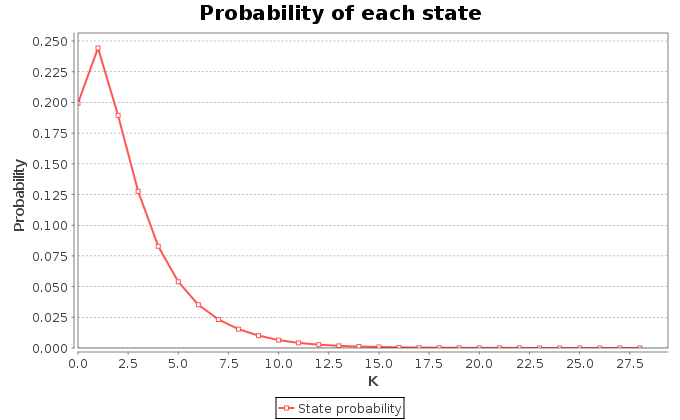
\includegraphics[width=\textwidth]{figures/mg1k.png}
	\end{center}}
	\caption{Probabilit`a di stato $k$, $\rho=0.8$, $\mu=1$, $N=100$, $arrivi=1000$ (Deterministic service time) }
	\label{fig:mg1k}
\end{figure}

All'utente viene lasciata la libert\`a di definire il grado di occupazione del servitore del sistema $\rho$, il tempo medio di servizio $\mu$, il numero di run da effettare $N$, il numero di arrivi per ciascuna run e, ovviamente, la tipologia di distribuzione. 

Come dati esemplificativi di questa gamma di simulazioni sono stati scelti quelli rappresentati in fig. \ref{fig:mg1k}, che descrive la probabilit\`a di stato di un sistema con tempo di servizio deterministico, e quelli di fig. \ref{fig:paretok}, raffigurante le probabilit\`a di stato di un sistema con tempo di servizio distribuito secondo Pareto.
\`E possibile notare come, a causa della maggior variabilit\`a dei tempi di servizio, il sistema con traffico di Pareto raggiunga stati di congestione caratterizzati da un alto numero di utenti nel sistema. Le probabilit\`a di stato infatti, sono non nulle anche con k pari a qualche centinaio di utenti.

\begin{figure}[!h]{
	\begin{center}
	   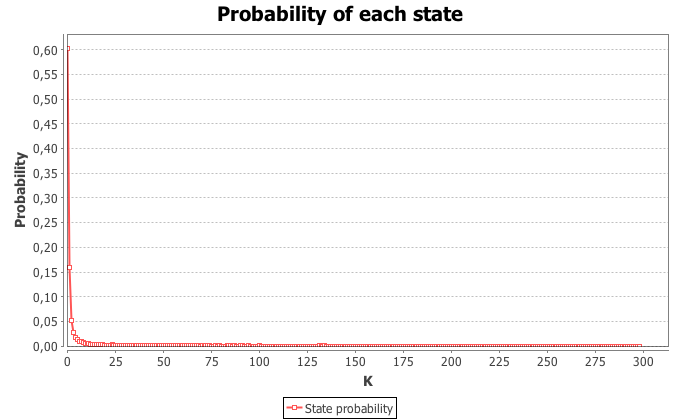
\includegraphics[width=\textwidth]{figures/statepareto.png}
	\end{center}}
	\caption{Probabilit`a di stato $k$, $\rho=0.5$, $\mu=2$, $N=100$, $arrivi=1000$ (Pareto service time) }
	\label{fig:paretok}
\end{figure}

\subsection{Analisi tecnica}

Analogamente a quanto visto in tutti casi precedenti ed in aderenza al modello definito per il simulatore, dopo un prima parte di handling da parte del pannello relativo all'interno dell'interfaccia grafica (classe {\tt MG1Panel}), si ricorre alla classe {\tt SimulationRunners}, ed in particolare al suo metodo:

$\cdot$ {\tt simulateMG1EvaluatingProbability(...)} \\
per l'esecuzione effettiva, mostrando il grafico di $P(k)$ in conclusione.

Tale metodo, per funzionare correttamente, si appoggia sul gi\`a precedentemente descritto {\tt FCFSSimulator}, utilizzato qu\`i con una sola classe di priorit\`a (quindi una singola coda di attesa), il quale fornisce un metodo ad-hoc, {\tt getStatesProbability}, che restituisce, per ogni stato $K(t)$ raggiunto durante la simulazione, la sua probabilit\`a empirica, calcolata semplicemente tenendo traccia del tempo totale trascorso in quel particolare stato, diviso per il tempo totale della simulazione.

\newpage
\section{Sistema $M/G/1$ con politica \emph{ Shortest Job Next}}

Come seconda simulazione opzionale si \`e scelto di implementare un sistema a coda con politica di tipo {\em shortest job first}. 

In questo caso all'utente viene chiesto di determinare, oltre agli usuali parametri di simulazione, il numero di step da considerare ed un moltiplicatore di $\theta$ al fine di eseguire la discretizzazione logaritmica dei tempi di servizio degli utenti del sistema in funzione della costruzione del grafico visualizzato al termine dell'elaborazione.

Il moltiplicatore di $\theta$, in particolare, andr\`a a determinare l'estensione del grafico lungo l'asse delle ascisse influendo dunque sulla porzione di curva visualizzata.

\begin{figure}[!h]{
	\begin{center}
	   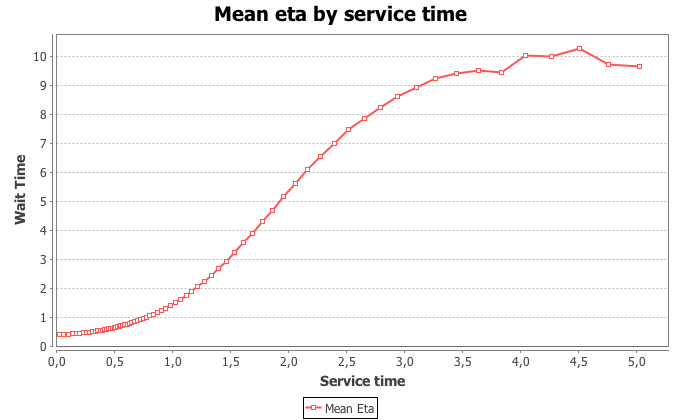
\includegraphics[width=\textwidth]{figures/MG1SJN[rho_08,mu_05,runs_1000,arrivals_100000,steps_30,mult_10].png}
	\end{center}}
	\caption{$\overline\eta$ in funzione del tempo di servizio $\theta$}
	\label{fig:mg1sjn}
\end{figure}

In figura \ref{fig:mg1sjn} \`e possibile osservare l'esito di una simulazione con parametri: $\rho=0.8$, $\mu=0.5$, $N=1000$, arrivi$=100'000$, $0\rightarrow\theta$ steps$=30$ ed intervallo di considerazione pari a $10\theta$: si noti come attraverso la discretizzazione logaritmica gli intervalli siano pi\`u concentrati e di dimensioni pi\`u ridotte intorno alla media (2) e di dimensioni maggiori man mano che ci si allontana dalla stessa.

\subsection{Note sulla discretizzazione logaritmica}
Al fine di ottenere simulazioni pi\`u accurate, l'intervallo continuo $\theta$ viene discretizzato, anzich\`e mediante una classica funzione lineare, ricorrendo ad una pi\`u complessa funzione logaritmica in modo tale da avere una maggiore concentrazione di piccoli intervalli nell'intorno della media di $\theta$  stesso, dove \`e pi\`u probabile ottenere valori, e pochi intervalli sempre pi\`u grandi mano a mano che ci si allontana da $\overline{\theta}$. La funzione utilizzata risulta essere la seguente: \\

$f(x) =	\left\{ \begin{array}{rcl}  
	-\log(-x+\overline{\theta}+b) + a + \overline{\theta} & \mbox{for} & x<\theta \\ 
	\log(+x-\overline{\theta}+b) - a + \overline{\theta} & \mbox{for} & x\geq\theta \\ 
	a = \overline{\theta}\cdot \frac{10^{-\overline{\theta}}}{1 - 10^{-\overline{\theta}}} & & \\ 
	b = log(a) \end{array} 
 \right.$ 	\\

parametrizzata rispetto a $\overline{\theta}$, $a$ e $b$; dove 
\begin{itemize}
\item $\overline{\theta}$ \`e la media attorno alla quale i valori di $\theta$ si dispongono
\item i parametri $a$ e $b$ dipendono da $\overline{\theta}$ e servono per forzare la funzione $f(x)$ a passare dai punti $(0,0)$ e $(\overline{\theta},\overline{\theta})$
\end{itemize}

Utilizzando una scala lineare lungo l'asse delle $y$, con passo costante e arbitrariamente definibile, e calcolandosi i relativi valori di $x$ mediante $f^{-1}(y)$ si ottengono i suddetti intervalli concentrati attorno al valore di $\overline{\theta}$; il valore scelto come rappresentativo di ciascun intervallo \`e semplicemente il valore mediano $x_{c} = \frac{x_{i} + x_{i + 1}}{2}$ \\

\begin{figure}[!h]{
	\begin{center}
	   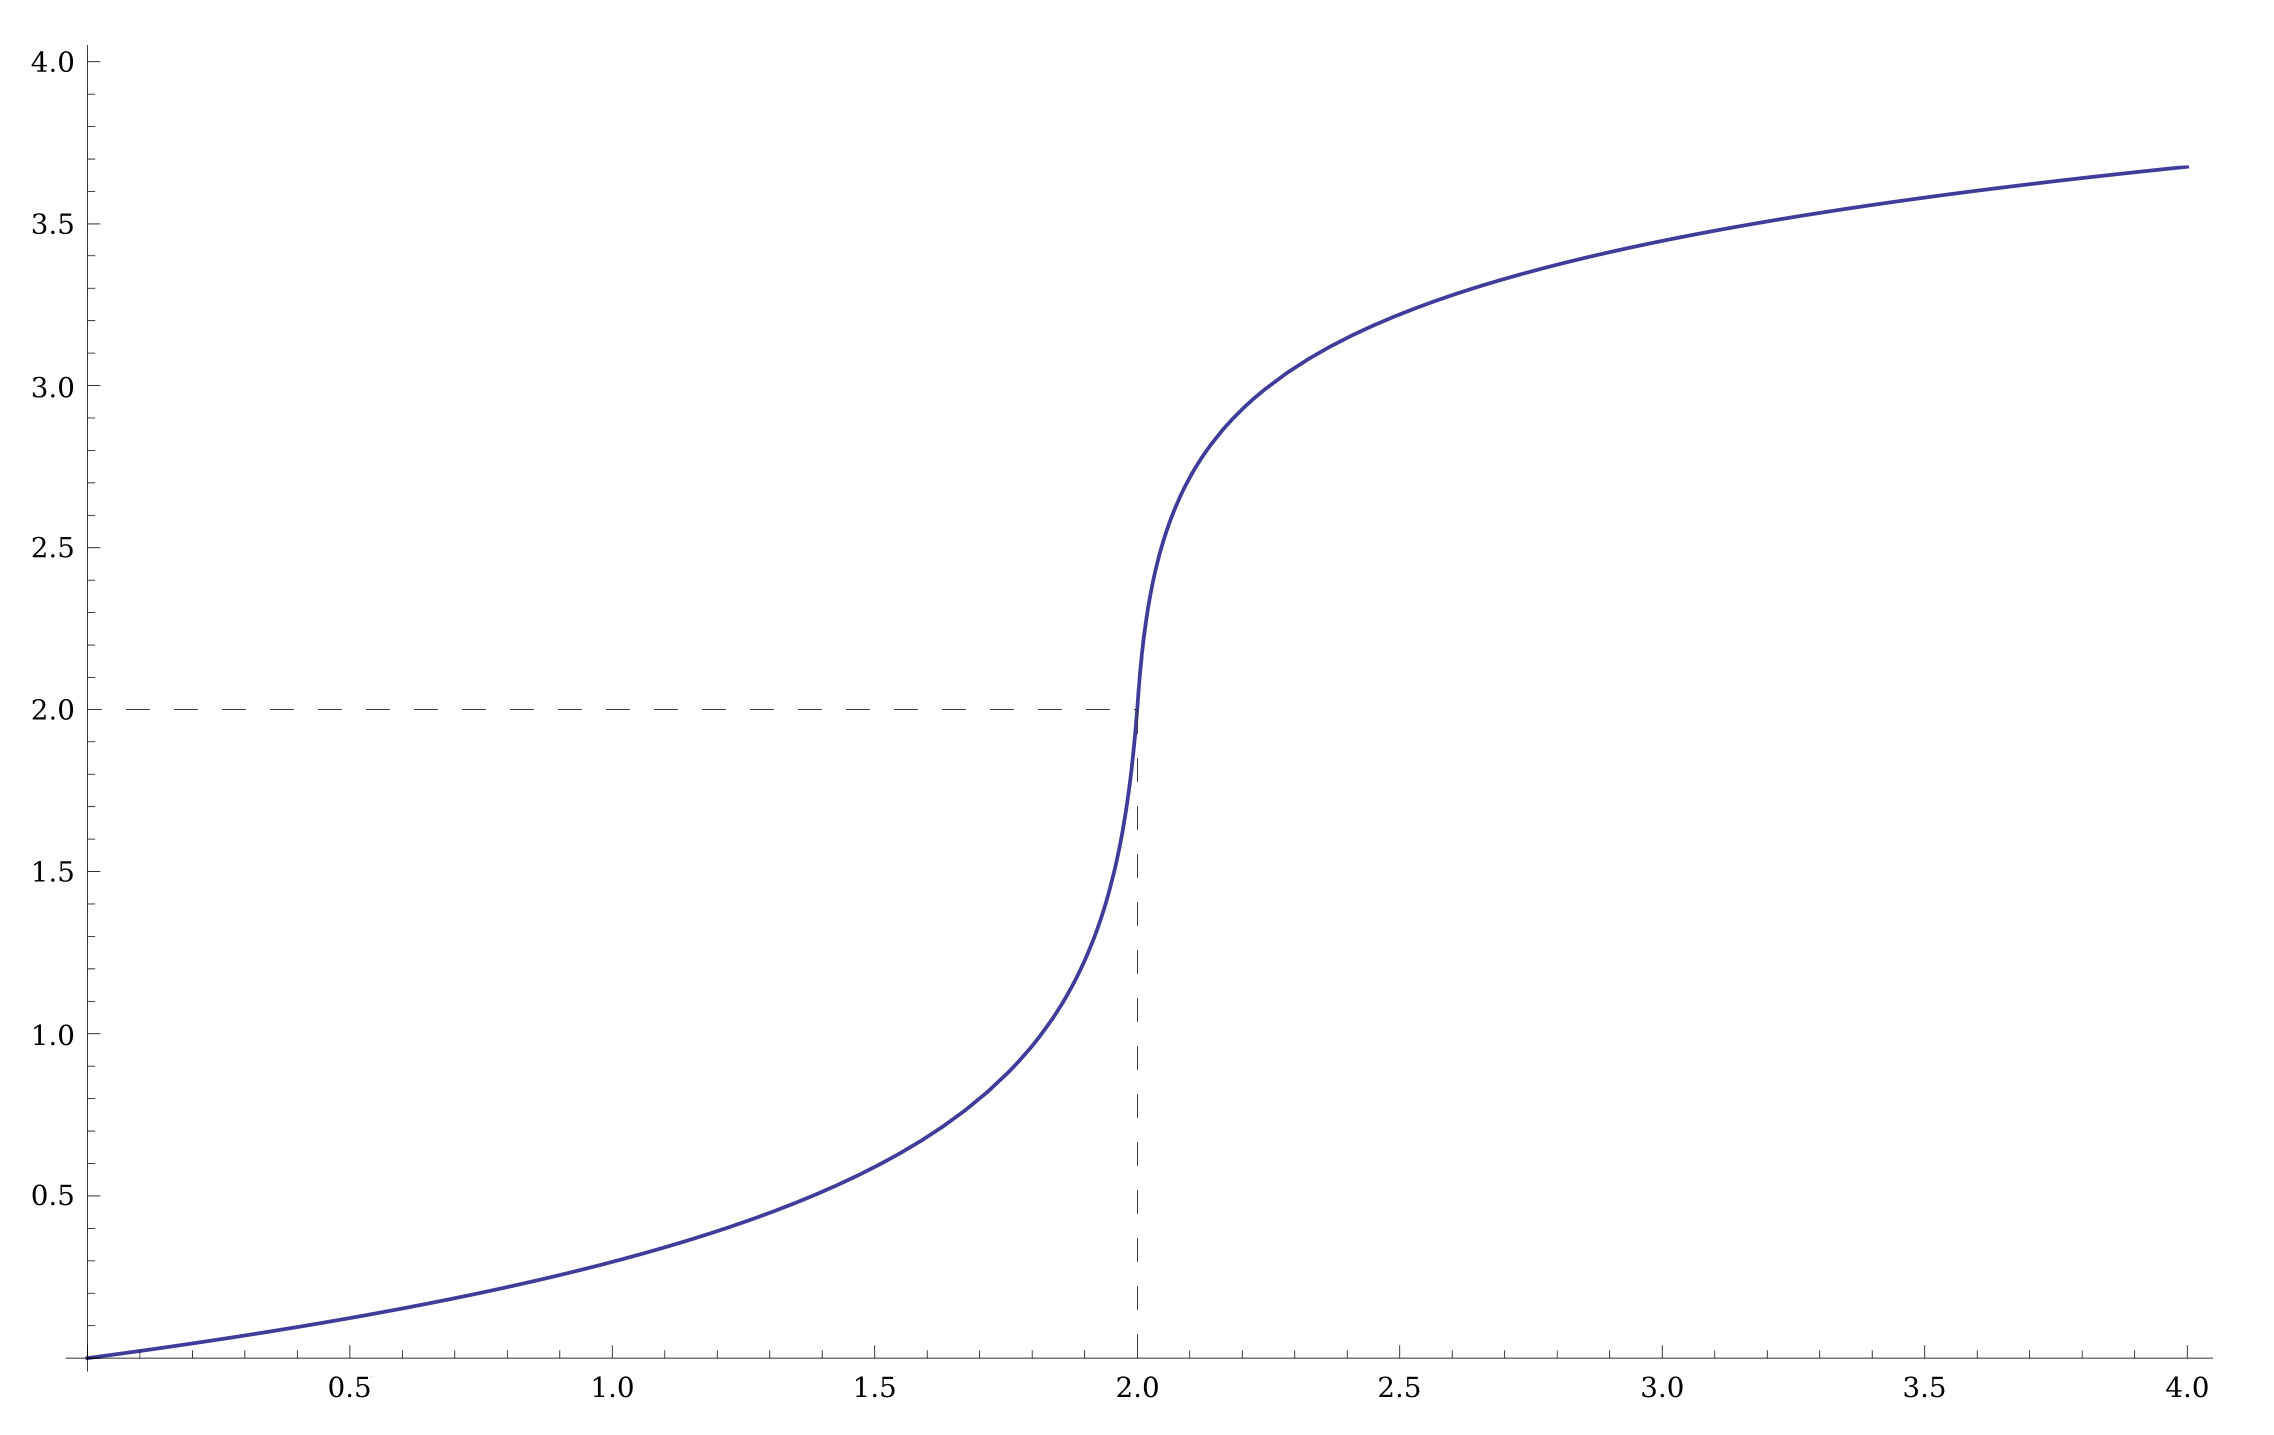
\includegraphics[width=\textwidth]{figures/loga-ritmo-per-ballare.png}
	\end{center}}
	\caption{esempio di una funzione logaritmica usata per la discretizzazione nel caso di $\overline{\theta} = 2$}
	\label{fig:log}
\end{figure}

\subsection{Analisi tecnica}

Nei casi precedenti, l'utilizzo (indiretto) della classe astratta {\tt Simulator} era sempre avvenuto attraverso la sua specializzazione {\tt FCFSSimulator}, sulla quale \`e stata implementata una gestiene di tipo FIFO.

Per la diversa tipologia di politica si \`e quindi provveduto all'implementazione della classe {\tt SJNSimulator}, che unitamente al metodo {\tt simulateMG1SJN(...)} della classe {\tt SimulationRunners} permette la definizione della nuova dinamica all'interno del sistema.

La classe {\tt SJNSimulator} concretizza la classe astratta {\tt Simulator} e, analogamente alla classe {\tt FCFSSimulator}, utilizza un'apposita specializzazione di {\tt ComparableEvent}, {\tt ServiceTimeComparedEvent}, la quale adotta come criterio di ordinamento il {\tt ServiceTime} di ciascun evento: eventi pi\'u corti verranno serviti prima. Una differenza importante rispetto al FCFSSimulator risiede nel calcolo dell'$\overline{\eta}$ per ciascuna \emph{classe}: infatti in questo caso, la coda di attesa \`e unica, non esistono priorit\`a differenti, ma viene richiesto di tenere traccia dei differenti tempi di attesa in base ad una discretizzazione dell'intervallo del tempo di servizio, $\theta$. A questo fine, ad ogni tempo di servizio, tramite la classe {\tt LogaritmicQuantizator}, viene assegnata una classe di appartenenza, con la quale aggiornare il relativo valore di attesa in coda.

\subsubsection{Nota finale}
Per ulteriori dettagli tecnici sull'implementazione del simulatore si rimanda alla consultazione della documentazione specifica (javadoc) contestualmente prodotta.
